\chapter{I Asked Robert Herjavec How He Made \$500 Million}

This chapter follows Lecture 33 of the School of Hard Knocks interview series, curated by LazyingArt LLC. The lecture begins in teaser form, not in explanatory form. We are given sale prices, annual earnings, luxury markers, and one sentence that functions as the chapter's organizing riddle: one may be rich without yet being wealthy. The Beverly Hills interviews that follow are therefore not incidental street color. They are the lecture's way of collecting local mechanisms before Robert Herjavec arrives to state the distinction more cleanly. We should read the chapter in that same order: first the puzzle, then the field evidence, then the arithmetic, and only after that the broader operating doctrine.

\section{Cold Open: Rich and Wealthy}

The opening montage does not argue. It points. One company is sold for \$30 million; another, we are told, for many hundreds of millions; a television network goes to News Corp; a product line becomes the biggest seller GNC had at the time; a year of roughly \$17 million is mentioned; and then the crucial line appears: ``I'm not rich. I'm wealthy.'' The lecture wants curiosity before doctrine. It wants us to feel that not all large numbers mean the same thing.

To keep the later discussion precise, we introduce a small set of objects that will recur throughout the chapter.

\begin{definition}
We write
\begin{align}
Y &= \text{annual income},\\
A &= \text{an owned asset or business},\\
V(A) &= \text{the realizable sale value of }A,\\
G_{\mathrm{exit}} &= \text{gain realized through an exit or sale},\\
W &= \text{wealth as durable command over assets and retained gains}.
\end{align}
\end{definition}

The teaser is then compressed by the first formal distinction:
\begin{equation}
W \not\equiv Y.
\end{equation}
A large \(Y\) may already be impressive, but the lecture is clearly pointing toward a second quantity, namely value locked inside an owned thing:
\begin{equation}
W \text{ depends on income, but it changes scale when } V(A) \text{ is realized through } G_{\mathrm{exit}}.
\end{equation}
At the beginning, however, this remains only a provocation. The lecture does not yet solve it. Instead, it moves into Beverly Hills and asks how different operators talk when asked, in public and at speed, how they became wealthy.

\section{Beverly Hills as a Wealth Field}

The host announces the method very plainly. Before meeting Herjavec, he will ask the people already moving through Beverly Hills what they did to become wealthy. This is an important structural choice. The lecture could have taken the shortcut of beginning with the famous case. Instead, it builds a field of comparison. Rodeo Drive and the surrounding streets become a dense money field in which different wealth grammars can be heard in compressed form.

Three such grammars emerge almost immediately:
\begin{itemize}
\item wealth through exits, where a company, network, or product is built and later sold;
\item wealth through operation, where an investor or founder screens businesses, times crises, and tries to add value to what is missing;
\item wealth through market positioning, where demand is recognized, competition is re-read, and the offer is made meaningfully different.
\end{itemize}

This is why the prelude cannot be collapsed into filler. It lowers the level of abstraction. It teaches us how the lecture wants to move. We do not begin with a theorem about wealth. We begin by listening to several operators describe how wealth actually appears in practice: through fitness, education, media, promotion, direct response, and investing. The lecture's later arithmetic will then sound less like an imported formula and more like a consolidation of the evidence already gathered.

\section{Action, Health, and the Cost of Inaction}

The first substantial street case is Body by Jake, and the lecture immediately performs an inversion. At first sight we have visible success: age held in check by discipline, bodily fitness, business longevity, and the glamour that naturally clings to such a figure. But the exchange itself moves away from appearance almost at once. Jake speaks about risk, about taking shots, about the partner who remains with the entrepreneur through instability, and about the emotional quality of decisive action.

This is the lecture's first deep shift. Health is mentioned, even jokingly, as a kind of wealth. Yet the real subject is not health for its own sake. It is the discipline to act and the refusal to become paralyzed by the possibility of loss. Jake says plainly that an entrepreneur wins some and loses some. The point is not invulnerability. The point is to avoid a later life in which unrealized ideas have hardened into a private accusation.

\subsection{Question \& Answer}

\paragraph{Question.} What is the cost of not acting on an idea?

\paragraph{Answer.} In this lecture the cost is not measured only by foregone revenue. The deeper cost is deferred self-judgment. When Jake says that the most valuable real estate lies in graveyards, he is not merely being dramatic. He is identifying a different loss function. What destroys us is not only failure in action, but also the accumulated memory of ideas we never had the courage to test.

The same interview then folds the action theme into a stronger question of identity. Jake recalls selling Fit TV to News Corp, but when he is asked what guiding principle he would leave to his son after his house burned down in the Palisades fire, he does not answer with cars, deal size, or accumulated property. He answers with a diagnostic: what are you made of? The lecture is telling us, well before Herjavec arrives, that material signs can disappear. What remains is the operating character that can generate again.

His final commercial rule in this segment, ``No is halfway to yes,'' belongs in the same family. It is not a mathematical law. It is a discipline of interpretation. Refusal is not necessarily terminal information. It is resistance that must be worked through.

\section{Screening, Crisis, and Product Differentiation}

The next operator shifts the lecture from existential cost to business criteria. He introduces himself as an investor in higher education; the transcript renders the college name as Theoria Technical College in Carlsbad, California. The exact orthography may be checked elsewhere if necessary, but the mechanism inside the interview is clear enough. He loves the field, owns institutions in it, and describes what he looks for when evaluating a company or founder.

\begin{equation}
I_{\mathrm{people}} + I_{\mathrm{processes}} + I_{\mathrm{profitability}} \lesssim 2,
\qquad
I_{\bullet} \in \{0,1\}.
\end{equation}

This is a careful reconstruction of his claim that most companies have two of the three. The usefulness of the form is immediate. The underwriting question is no longer whether a firm is complete in every direction. The question becomes: which leg is missing, and is that missing leg something the investor can supply?

\begin{figure}
\centering
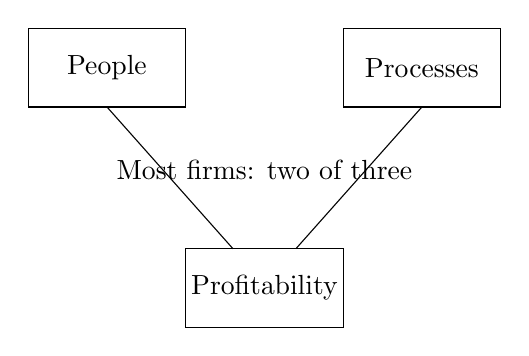
\begin{tikzpicture}
\draw (-3,1) rectangle (-1,2);
\node at (-2,1.5) {People};
\draw (1,1) rectangle (3,2);
\node at (2,1.5) {Processes};
\draw (-1,-1.8) rectangle (1,-0.8);
\node at (0,-1.3) {Profitability};
\draw (-2,1) -- (-0.4,-0.8);
\draw (2,1) -- (0.4,-0.8);
\node at (0,0.2) {Most firms: two of three};
\end{tikzpicture}
\end{figure}

The host then asks the right follow-up question: what happened in the year when this operator made about \$17 million? The lecture's rhythm matters here. It does not leave a large number uninterpreted. It demands the mechanism beneath the number. The answer is pandemic timing. When the world crashed, he says, he doubled down, helped businesses improve, and moved while others were fearful. In this lecture, fear and opportunity are repeatedly paired. Again, this is not a theorem; it is a directional commercial claim about timing and nerve.

The same operator then contributes a management heuristic through the so-called ``Obama effect.'' One need not be the smartest person in the room. One can instead gather strong people, speak last, and let the room contribute before the leader sets direction. The lecture thereby moves from personal action to organized action.

At this point the video pauses for a sponsor interlude about signing and closing documents. As a matter of doctrine, that interruption is not central. As a matter of rhythm, it is useful: it breaks the first cluster of street interviews and resets the lecture for one more warm-up case before Herjavec.

That final warm-up operator belongs to health products, promotion, and direct response. He ties his success to the first ``Herbal Viagra,'' to media, to sales letters, to books such as \textit{Think and Grow Rich} and Dan Kennedy's \textit{The Ultimate Sales Letter}, and above all to the problem of finding a winning product. His advice begins at the expected place: read, think, talk, network, keep the eyes open. But it becomes more interesting when the host asks about competition.

\begin{equation}
n_{\mathrm{competitors}} \uparrow
\quad \Rightarrow \quad
D_{\mathrm{market}} \uparrow
\end{equation}

This is the lecture's compact version of the gas-station argument: if many people are already selling in a market, that fact may reveal demand rather than forbid entry. Yet the lecture does not stop there. Competition proves activity, not our distinctiveness within activity. That is why the operator immediately adds the second clause: the offer must still be different. In his own story, the winning route was not merely to join a market, but to find a different product-processing angle, connect it to strong media, and make the offer stand apart.

Thus the warm-up sequence gives us four tools before Herjavec speaks directly: act before regret calcifies; screen businesses by their missing leg; see crisis as an opening if one can still move; and read competition together with differentiation rather than against it.

\section{Rich, Wealthy, and the Arithmetic of Exit}

Only now does the lecture turn to Herjavec, and the delay is important. By the time he appears, the local mechanism bank has already been assembled. His interview therefore does not start from zero. It consolidates. The host even asks for this explicitly: no holding back, give us the secrets. The lecture now moves from sampling to grammar.

Asked what he saw early in cybersecurity and the internet, Herjavec answers with the chapter's decisive comparative claim:
\begin{align}
\text{follow a trend} &\to \text{get rich},\\
\text{create a trend} &\to \text{get wealthy}.
\end{align}
We should keep the asymmetry exact. Following monetizes participation. Creating monetizes control, category position, or early ownership. The sentence is already about value capture before it becomes explicitly about arithmetic.

He then turns to motive. Mark Cuban, he says, wanted to be rich at twelve. Herjavec, by contrast, wanted not to be poor. This shift matters because it changes the emotional engine of the whole lecture. One can be pulled by aspiration, but one can also be driven by refusal. That leads directly to the lecture's change axiom:
\begin{equation}
S_{t+1} \approx S_t
\qquad
\text{when}
\qquad
\Delta a_t = 0.
\end{equation}
This is a schematic rendering of ``Nothing changes if nothing changes.'' We introduce it here, and not earlier, because this is where the lecture itself finally states the rule outright. Action is no longer only brave or admirable. It becomes the necessary condition for state change.

\subsection{Question \& Answer}

\paragraph{Question.} Why can a person earn a very high income and still fail to become truly wealthy?

\paragraph{Answer.} Because income and realized ownership value are not the same thing. A large income can make us rich. Wealth, in the lecture's stronger sense, appears when we build something that stores value and can later be sold. The sale event is not just more of the same. It is a discontinuous realization of asset value.

Herjavec makes that distinction numerically explicit:
\begin{align}
M_{\mathrm{peak}} &= Y + G_{\mathrm{exit}},\\
M_{\mathrm{peak}} &\approx \$500\text{M},\\
Y &\approx \$18\text{M}.
\end{align}
Here \(M_{\mathrm{peak}}\) is the largest money year he names, \(Y\) is what he reports on an income basis, and \(G_{\mathrm{exit}}\) is the gain associated with the sale of a business. The transcript does not give us a full accounting statement, but it gives us enough to preserve the conceptual split faithfully.

\paragraph{Worked example.} At the level of lecture arithmetic, we may isolate the exit component directly.
\begin{enumerate}
\item Begin from \(M_{\mathrm{peak}} = Y + G_{\mathrm{exit}}\).
\item Substitute \(M_{\mathrm{peak}} \approx \$500\text{M}\) and \(Y \approx \$18\text{M}\).
\item Subtract to identify the dominant term.
\end{enumerate}
Thus
\begin{align}
G_{\mathrm{exit}}
&\approx M_{\mathrm{peak}} - Y \\
&\approx \$500\text{M} - \$18\text{M} \\
&\approx \$482\text{M}.
\end{align}
The exact decomposition is not supplied in the lecture, so we keep the example approximate. But its pedagogical force is strong. The spectacular year is not salary-sized. It is exit-sized.

\begin{figure}
\centering
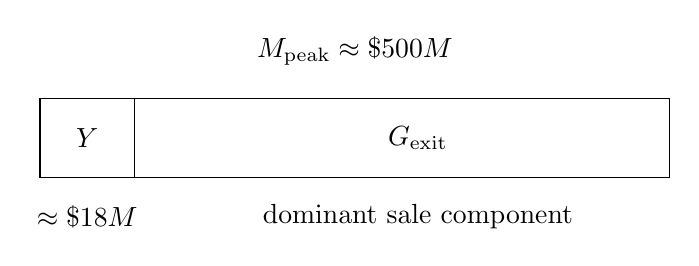
\begin{tikzpicture}
\draw (0,0) rectangle (8,1);
\draw (0,0) rectangle (1.2,1);
\node at (4,1.6) {$M_{\mathrm{peak}} \approx \$500\text{M}$};
\node at (0.6,0.5) {$Y$};
\node at (4.8,0.5) {$G_{\mathrm{exit}}$};
\node at (0.6,-0.5) {$\approx \$18\text{M}$};
\node at (4.8,-0.5) {dominant sale component};
\end{tikzpicture}
\end{figure}

This is only a schematic diagram, but it makes the lecture's opening teaser legible. The distinction between rich and wealthy is not moralistic. It is structural. Income may be large; wealth scales when a valuable asset is owned and then realized.

\section{Recovery, Real Estate, Sales, and Relationship Capital}

Once the wealth arithmetic has been stated, the lecture turns again and becomes rougher. Herjavec tells a betrayal story from his first company: a sales manager was stealing by splitting orders through a side business. The point of the story is not merely that bad actors exist. The point is that success does not remove bad days. Barbara Corcoran's rule, as reported by Herjavec, is that the operative difference is how long we wallow in misery. Herjavec allows himself the bad moment, even the crying, but not the indefinite stay. Then he gets up and works again. Elon Musk's line about eating glass and staring into the abyss is placed here to make the emotional register unmistakable.

From recovery the lecture moves into durable assets. Charlie Munger, as Herjavec reports him, advises never selling a house. Herjavec translates that maxim into a holding-horizon doctrine:
\begin{equation}
H_{\mathrm{RE}} \ge 10 \text{ years}
\quad \Rightarrow \quad
\Pi_{\mathrm{RE}} > 0.
\end{equation}
He then names the real danger with equal clarity:
\begin{equation}
H_{\mathrm{RE}} < 10 \text{ years}
\quad \text{together with liquidity pressure}
\end{equation}
is what forces the loss. Time, in other words, is part of the asset. The problem is not simply price; it is whether we are able to keep the position alive long enough for time to do its work.

The lecture then asks for a sales masterclass, and Herjavec responds by refusing the usual theatrical answer. Before one teaches selling, one must first identify the buyer. One pitch for everybody is the central mistake. The sequence can be rendered as
\begin{equation}
p_{\mathrm{close}} = p(N,P),
\qquad
N \text{ before } P.
\end{equation}
Need discovery comes first; pitch comes second.

\begin{figure}
\centering
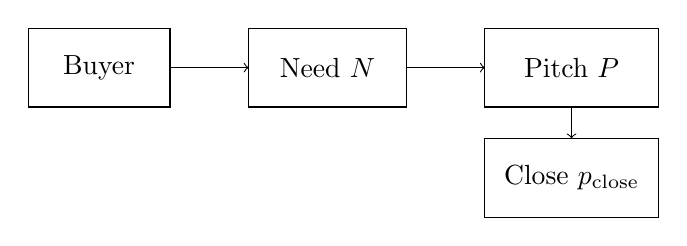
\begin{tikzpicture}
\draw (-4,0) rectangle (-2.2,1);
\node at (-3.1,0.5) {Buyer};
\draw (-1.2,0) rectangle (0.8,1);
\node at (-0.2,0.5) {Need \(N\)};
\draw (1.8,0) rectangle (4,1);
\node at (2.9,0.5) {Pitch \(P\)};
\draw[->] (-2.2,0.5) -- (-1.2,0.5);
\draw[->] (0.8,0.5) -- (1.8,0.5);
\draw (1.8,-1.4) rectangle (4,-0.4);
\node at (2.9,-0.9) {Close \(p_{\mathrm{close}}\)};
\draw[->] (2.9,0) -- (2.9,-0.4);
\end{tikzpicture}
\end{figure}

\subsection{Question \& Answer}

\paragraph{Question.} What actually makes someone willing to buy from us?

\paragraph{Answer.} The lecture gives two answers, and we should keep them together. First, the offer must answer a real need. Second, the buyer must feel something good in the exchange. The late instruction ``Sell joy'' is not separate from the sales lesson; it completes it. We do not sell by information alone. We sell by matching need and shaping feeling.

From sales the lecture moves into access. Asked whether what matters is what we know or who we know, Herjavec rejects the passive folklore of networking. If one starts with little money and few connections, one must become someone worth knowing. That gives us the chapter's update rule for relationship capital:
\begin{equation}
C_{t+1} = f(C_t,V_t),
\end{equation}
where \(C_t\) is connection capital and \(V_t\) is the visible value we provide. This is a stronger formulation than ``go meet important people.'' It says that access is built by becoming useful, interesting, or otherwise valuable enough that stronger people have a reason to engage.

The lecture then names obsession as the common trait of ultra-successful operators. Passion fades too easily. Obsession persists. It also allows a person to see not merely the world as it is, but the world as it might be forced to become. We should hear an echo here of the earlier Body by Jake segment. The lecture keeps circling back to the same question: what kind of person continues to act under uncertainty?

At this point the health motif returns in a sharper form. Herjavec says that the biggest flex of wealth today is not the car or the jet, but being in shape. The point is no longer ornamental. Wealth is being evaluated by what it permits us to preserve.

The next branch concerns starting conditions:
\begin{align}
K_0 > 0 &\Rightarrow \text{use capital as leverage and barrier to entry},\\
K_0 \approx 0 &\Rightarrow \text{favor e-commerce and brand-building}.
\end{align}
Commercial buildings, data centers, and land sit on the first side. E-commerce and online brand construction sit on the second. The lecture does not romanticize one path over the other. It simply insists that strategy follow capitalization.

Herjavec then restates the human-capital priority in the simplest possible form:
\begin{equation}
(\text{good operator},\text{bad idea})
\succ
(\text{bad operator},\text{good business}).
\end{equation}
He says he invests in people, always. The inequality is only ordinal, but it is exact enough to preserve the lecture's judgment.

The Mark Cuban ``man in the t-shirt'' anecdote extends the same logic into social signaling. The dangerous person in the room is not the one dressed to impress. It is the one who no longer needs to dress for permission. The signal of wealth here is freedom from signaling. That, too, is a form of accumulated position.

Only after all this does the lecture pivot to AI. If Herjavec lost everything but kept his contact book, he says he would build an AI company. He favors infrastructure over the merely consumer layer, and his practical advice is to train the model to the way one already works. This keeps AI inside the larger logic of the chapter. The tool is valuable when it compounds an operator's existing pattern rather than replacing the need for one.

The final movement of the lecture is therefore not a new theorem, but a human completion. ``Sell joy.'' ``It's not what you say, it's how you make people feel.'' The priest's line about the fascination of another human being re-enters here and locks the chapter shut. Wealth may be created through ownership, exits, and durable assets, but every one of those processes still runs through human beings with stories, emotions, and memories. The lecture does not end by leaving arithmetic behind. It ends by telling us what arithmetic alone cannot do.

\section{Summary}

The chapter opens with teaser numbers and ends with a much clearer distinction. To be rich is not yet to be wealthy, because income and realized ownership value are not the same category of thing. The Beverly Hills prelude matters precisely because it lets us watch that distinction emerge indirectly through local cases: action against regret, partnership under risk, screening by missing legs, crisis as opening, and differentiation inside crowded markets. Herjavec then names the arithmetic explicitly: peak money comes from income plus exit gain, and the scale of wealth changes when a valuable asset is sold. The later doctrine extends rather than replaces that arithmetic. Recover quickly, hold long enough, discover need before pitching, build access by providing value, prefer people over ideas, and remember that even in the hard mechanics of wealth-building the final medium of business is still the human encounter.